\documentclass[10pt, a4paper, twocolumn]{article}

% ---------- Fonts (standard academic: Palatino + math) ----------
\usepackage[T1]{fontenc}
\usepackage[utf8]{inputenc}
\usepackage{mathpazo}
\usepackage[scaled=0.95]{helvet}
\usepackage{courier}
\usepackage[english]{babel}

% ---------- Page layout ----------
\usepackage[a4paper, margin=0.5in, columnsep=0.25in]{geometry}

% ---------- Typography ----------
\setlength{\parindent}{0pt}
\setlength{\parskip}{4pt}
\usepackage{setspace}

% ---------- Graphics and colors ----------
\usepackage{graphicx}
\usepackage{xcolor}
\usepackage{float}
\usepackage{tikz}
\usetikzlibrary{positioning, arrows.meta}

% ---------- Math and tables ----------
\usepackage{amsmath, amssymb}
\usepackage{booktabs}

% ---------- Lists ----------
\usepackage{enumitem}
\setlist{nosep}

% ---------- Captions ----------
\usepackage{caption}
\usepackage{subcaption}

% ---------- Code ----------
\usepackage{listings}

% ---------- Hyperlinks ----------
\usepackage{hyperref}
\hypersetup{
  pdfborder = 0 0 0,
  colorlinks = true,
  linkcolor = black,
  citecolor = black,
  urlcolor = black
}

% ---------- References ----------
\usepackage[numbers]{natbib}
\usepackage{tocbibind}
\usepackage{url}

% ---------- Headers / Footers ----------
\usepackage{fancyhdr}
\usepackage{titlesec}
\usepackage{titling}

% ---------- Header / Footer ----------
\pagestyle{fancy}
\fancyhf{}
\fancyhead[L]{\footnotesize\itshape DeVi Comfort \textbullet{} 2026}
\fancyhead[R]{\footnotesize\thepage}
\renewcommand{\headrulewidth}{0.4pt}
\renewcommand{\footrulewidth}{0pt}

% ---------- Title ----------
\title{Internship Research Report Period 1 and 2}
\author{Nout Mulder}
\date{2026}

% ---------- Document ----------
\begin{document}

% ---------- Journal-style Title Block (full width) ----------
\twocolumn[
\thispagestyle{fancy}
\vspace*{0.3cm}
{\small\itshape Internship Report DeVi Comfort. 2026; 1(1): 1--\pageref{LastPage}\par}
\vspace{0.2cm}
\hrule
\vspace{0.5cm}
\begin{center}
{\Large\bfseries DEVELOPING A LIVE 3D TELEMETRY VISUALIZATION\\FOR STAIRLIFT FAULT DIAGNOSIS\par}
\vspace{0.3cm}
{\normalsize Nout Mulder\par}
\vspace{0.1cm}
{\small DeVi Comfort \textbullet{} Engineering \textbullet{} Opmeer\par}
\end{center}
\vspace{0.3cm}
\hrule
\vspace{0.4cm}

\begin{center}
\begin{minipage}{0.9\textwidth}
\small
\textbf{Abstract.}
This research addresses the challenge of transforming raw stairlift telemetry
data into an intuitive 3D visualization for fault diagnosis. The core technical
problem is the live mapping of noisy, asynchronous sensor readings onto a
curved 3D rail geometry with segment-dependent encoder-to-distance ratios. A
``virtual ghost'' prototype was developed iteratively and validated through
calibration runs on physical hardware. The results show that a processing
pipeline combining non-linear encoder mapping, recursive state estimation, and
smooth tangent-based orientation reconstruction produces a stable live 3D
representation. This enables faster spatial interpretation of stairlift
position and fault conditions compared to text-based error codes.
\end{minipage}
\end{center}
\vspace{0.3cm}
\hrule
\vspace{0.5cm}
] % end of \twocolumn[...]

% ============================================================
\section{Introduction}
\label{sec:introduction}

DeVi Comfort designs and manufactures stairlift systems and develops the
accompanying control software in-house. A stairlift consists of a chair unit
that travels along a custom-bent rail mounted to a staircase. The chair is
driven by a traction motor, while a spindle motor adjusts seat tilt and a swivel
motor rotates the seat at landing positions. During operation, embedded
controllers continuously produce telemetry: traction encoder pulses, spindle
encoder values, swivel angles, and system status bits including error codes.
For service, maintenance, and further development, engineers need to quickly
understand the current state of a stairlift: where the chair is positioned on
the rail, whether it is moving correctly, and what deviations or faults have
occurred.

Currently, fault information from the controller is presented as textual error
codes and numeric status values. While technically correct, these require
significant domain knowledge to interpret spatially. An error code indicating a
position deviation does not convey where on the rail the deviation occurred, in
which direction, or how large the discrepancy is.

The underlying technical challenge is twofold. The raw telemetry data (encoder
pulse counts, spindle values, swivel angles) must be mapped onto a
three-dimensional rail geometry. This rail contains straight sections, vertical
bends, and horizontal bends, each consuming a different number of encoder pulses
per millimeter of travel. Additionally, the sensor readings arrive at irregular
intervals over a wireless serial link with noise, latency, and occasional packet
loss. The visualization must bridge the gap between these asynchronous
measurements and a continuous, smooth spatial representation that updates at
display frame rate.

A live 3D visualization of stairlift position and movement would have direct
practical value. Service engineers could visually identify whether the chair has
lost its expected position, is stuck in a bend, or exhibits abnormal tilt. This
would reduce diagnosis time and minimize unnecessary on-site visits. For the
development team, a live telemetry view would enable rapid verification of
firmware behavior during testing and commissioning of new rail configurations.

The goal of this research is to determine which data processing and mathematical
models are needed to transform live stairlift telemetry into a reliable and
intuitive 3D visualization for fault analysis. The central research question is:

\textit{What data processing pipeline and mathematical models are required to
transform live stairlift telemetry into a 3D visualization that enables faster
and more intuitive fault diagnosis compared to text-based error codes?}

The research follows an iterative prototyping approach based on the spiral
model~\cite{boehm1988spiral}. Each iteration consists of analysis, design,
implementation, and validation against practical scenarios on physical hardware.
The primary methods are formal mathematical analysis, architectural design, and
experiment with measurable accuracy criteria.

Section~\ref{sec:problem-statement} presents the problem statement, structured
as a problem analysis, prior work survey, and the resulting research questions.
Section~\ref{sec:methods} describes the research methods per subquestion.
Section~\ref{sec:results} presents the findings. Section~\ref{sec:conclusion}
concludes with answers to the research questions and recommendations.

% ============================================================
\section{Problem Statement}
\label{sec:problem-statement}

\subsection{Problem Analysis}
\label{sec:problem-analysis}

\subsubsection{Sensor-to-Spatial Mapping in Mechatronic Systems}
The challenge of transforming discrete sensor readings into a continuous spatial
representation is well-established in mechatronic system
diagnostics~\cite{grieves2017digitaltwin}. In the broader context of digital
twin research, Bofill et al.\ identify real-time sensor data integration as one
of the primary technical barriers to effective fault
monitoring~\cite{bofill2023digitaltwin}. The fundamental difficulty is that
sensors produce scalar values (counts, voltages, status bits) at discrete
intervals, while a spatial visualization requires a continuous 3D position and
orientation that updates at display frame rate.

In robotics and vehicle tracking, this problem is typically simplified by the
assumption that sensor readings map linearly to spatial
coordinates~\cite{elmenreich2002sensorfusion}. A rotary encoder on a linear
actuator, for example, produces pulses proportional to displacement, and the
mapping from pulse count to position is a single constant. This assumption
breaks down when the trajectory is non-linear: on a curved path, the
relationship between encoder pulses and spatial displacement depends on the
local curvature~\cite{merry2013encoder}.

\subsubsection{Non-Linear Encoder Mapping on Curved Rails}
A stairlift rail is composed of straight sections, vertical bends (pitch
changes), and horizontal bends (yaw changes). The mechanical drive system uses a
traction motor with an incremental encoder to measure
displacement~\cite{bolton2019mechatronics}. Due to the geometry of the rail
bending mechanism, each segment type consumes a different number of encoder
pulses per unit of physical travel. A vertical upward bend, for instance,
requires fewer pulses per millimeter of arc length than a downward bend, because
the traction wheel follows the inner or outer radius of the curve respectively.

This means that a single scalar encoder reading cannot be converted to a 3D
position without a model of the full rail topology. The mapping must account for
the cumulative pulse cost of each preceding segment, making it a piecewise
non-linear function rather than a simple linear scaling. Without such a model,
position errors accumulate at every bend transition, growing proportionally to
the number of bends in the rail.

\subsubsection{State Estimation from Noisy Telemetry}
The telemetry link between the stairlift controller and the visualization
application introduces additional challenges. The Bluetooth Classic Serial Port
Profile~\cite{bluetoothsig2022spp} provides a virtual serial connection at
approximately 20\,Hz, but with variable latency (10--80\,ms per round trip) and
occasional packet loss. The visualization, however, must render at 60\,fps
(16.7\,ms per frame).

This creates a temporal mismatch: new sensor data arrives roughly every third
frame, and frames between measurements must be filled with predicted values. If
the most recent measurement is simply held constant until the next arrives, the
display exhibits visible staircase-like jumps. If measurements are used directly
without filtering, encoder quantization noise (inherent to incremental
encoders~\cite{merry2013encoder}) causes jitter. Both artifacts undermine the
interpretability of the visualization.

The general solution to this class of problem is recursive state estimation: a
filter that maintains a probabilistic model of the system state and updates it
with each new measurement~\cite{kalman1960}. The choice of filter, its process
model, and its tuning determine the trade-off between responsiveness and
smoothness.

\subsubsection{Multi-Axis Orientation from Independent Sensors}
The stairlift chair has four independent rotational degrees of freedom: yaw
(direction along the rail), pitch (rail inclination), seat tilt (spindle motor),
and seat rotation (swivel motor). Each is measured by a separate sensor with its
own update rate and noise characteristics. Reconstructing the full 3D
orientation of the chair requires combining these independent streams into a
single consistent rotation, avoiding mathematical singularities that can occur
when multiple rotations are composed~\cite{shoemake1985quaternion}.

\subsubsection{Summary of Technical Subproblems}
Three interrelated technical subproblems emerge from this analysis:
\begin{enumerate}[leftmargin=*]
  \item \textbf{Non-linear encoder-to-position mapping:} Converting a scalar
    encoder count into a normalized position along a 3D curve with
    segment-dependent pulse costs.
  \item \textbf{State estimation:} Producing a smooth, low-latency
    estimate of position and velocity from noisy, asynchronous measurements
    arriving at a lower rate than the display refresh.
  \item \textbf{Multi-axis orientation reconstruction:} Combining four
    independent rotational sensor streams into a singularity-free 3D
    orientation.
\end{enumerate}

\subsection{Prior Work}
\label{sec:prior-work}

\subsubsection{State Estimation}
For state estimation from noisy sensor data, three approaches are commonly
used in embedded and robotics applications: moving average filters,
complementary filters, and Kalman filters.

A \textbf{moving average filter} computes the mean of the last $N$ samples and
outputs it as the filtered value. Smith shows that for purely time-domain
noise reduction on stationary or slowly varying signals, moving averages are
close to optimal and have the advantage of computational
simplicity~\cite{smith1997dsp}. They are therefore a strong choice for
applications where the input signal changes slowly relative to the sampling
rate and no prediction is required between samples. However, moving averages
introduce a latency proportional to the window size (effectively delaying the
signal by $N/2$ samples), cannot extrapolate between measurements, and perform
poorly on transient or fast-changing signals. For stairlift telemetry, where
sensor readings arrive at $\sim$20\,Hz but the display updates at 60\,fps,
pure moving-average smoothing cannot fill the inter-sample gap.

A \textbf{complementary filter} combines two sensor sources with complementary
frequency characteristics, typically using a low-pass filter on one source and
a high-pass filter on the other~\cite{narkhede2021cascaded}. This is the
standard approach in IMU fusion, where slow, drift-free accelerometer data is
combined with fast, noisy gyroscope data to estimate attitude. Complementary
filters are computationally light and do not require a statistical model of
the noise. They are therefore preferred in cost-constrained or high-rate
embedded systems with multiple complementary sensors. However, they assume
that two sensor sources are available with complementary frequency content,
which is not the case for the stairlift: the traction encoder is the only
direct position sensor, and its noise is not separable by frequency from its
signal.

The \textbf{Kalman filter} maintains a probabilistic estimate of system state
(position and velocity) and updates it with each new measurement, optimally
balancing prediction uncertainty against measurement
noise~\cite{kalman1960, welch1995kalman, bolton2019mechatronics}. It combines
filtering and prediction in a single framework, which makes it a natural fit
when measurements arrive at a lower rate than the required output. The cost
is higher computational complexity and the need to tune process and
measurement noise parameters. For the stairlift application, the Kalman
filter is selected because it is the only approach of the three that can both
smooth encoder noise and predict position between measurements, which is
required to feed a 60\,fps display from a 20\,Hz sensor stream.

\subsubsection{Spline Interpolation for Smooth Trajectories}
To produce smooth position and orientation transitions along a discrete set
of rail control points, interpolation is required. Three families of splines
are candidates.

\textbf{Linear interpolation} between adjacent points produces sharp direction
changes at segment boundaries (no $C^1$ continuity). It is computationally
cheap and is the right choice when the interpolated quantity is expected to
change piecewise linearly, or when downstream processing does not need a
continuous tangent. For visual orientation of a chair along a continuously
curved rail, the discontinuous tangent of linear interpolation would cause the
chair to visibly ``snap'' at each rail point.

\textbf{B-splines} (and their rational generalization, NURBS) are the de
facto standard in CAD and industrial curve design. They provide arbitrary
continuity ($C^k$) through the choice of degree, and local control
(moving one control point affects only a bounded region of the
curve)~\cite{piegl1991nurbs}. They are preferred when the curve itself is
being designed (CAD surfaces, font glyphs, animation paths) and the control
points are construction handles rather than fixed waypoints. Their disadvantage
for this application is that the curve does \emph{not} pass through the
control points, so it does not correspond to the physical rail geometry: the
ghost chair would follow a smoothed approximation of the rail rather than the
rail itself.

\textbf{Catmull-Rom splines} interpolate through each control point and
provide $C^1$ continuity at those points~\cite{catmullrom1974}. They are the
natural choice when the control points are fixed physical waypoints (as is
the case for the rail) and the primary goal is a smooth tangent for
orientation purposes. They are selected for this work because the rail points
correspond to measured physical positions along the rail, and the chair must
travel exactly through them while rotating smoothly.

\subsubsection{Rotation Representation}
Three representations of 3D rotation are in common use: Euler angles,
rotation matrices, and unit quaternions.

\textbf{Euler angles} (roll, pitch, yaw) are human-readable and require only
three parameters. Diebel notes that for systems with limited rotation ranges,
or where only a single rotation axis is actively used, Euler angles are a
reasonable and computationally inexpensive
choice~\cite{diebel2006attitude}. Many industrial applications (e.g.,
single-axis servo control, simple tilt sensors) use Euler angles without
issue. The well-known drawback is gimbal lock: when two rotation axes align,
one degree of freedom is lost and the inverse mapping becomes singular. For
the stairlift, with four independent rotational axes that can interact
(rail yaw, rail pitch, seat tilt, seat rotation), the risk of gimbal lock
during certain rail configurations is real.

\textbf{Rotation matrices} (3$\times$3 orthogonal matrices) are free of
singularities and compose cleanly, but require nine parameters with six
constraints, are costly to interpolate smoothly, and accumulate numerical
drift (loss of orthogonality) over many composed rotations. They are standard
in computer graphics shaders, where the GPU performs matrix operations
natively.

\textbf{Unit quaternions} (four parameters, one constraint) are free of
gimbal lock, compose compactly, and support smooth spherical linear
interpolation~\cite{shoemake1985quaternion}. They are the standard in
real-time graphics and robotics for full 3D orientation~\cite{kuipers1999quaternions,
diebel2006attitude}. For the stairlift chair, where four independent rotations
must be composed every frame without visual artifacts, quaternions are
selected to avoid the gimbal lock risk of Euler angles and the numerical
drift of rotation matrices.

\subsubsection{Real-Time 3D Engine Selection}
\label{sec:prior-engine}
The renderer layer of the pipeline (Section~\ref{sec:results-q2}) requires a
3D engine that meets four criteria: (C1) configurability for custom shaders,
(C2) cross-platform export to desktop and Android~12+ from a single source
tree, (C3) licence compatible with closed-source commercial deployment, and
(C4) native glTF binary import to match DeVi Comfort's CAD
pipeline~\cite{khronos2021gltf}. Table~\ref{tab:engine-mca} scores four
candidates against these criteria.

\begin{table}[H]
\centering
\caption{Multi-criteria comparison of real-time 3D engines against the criteria defined in Section~\ref{sec:prior-engine}. ``+'' indicates the criterion is fully met, ``='' partially, ``$-$'' not met.}
\label{tab:engine-mca}
\small
\begin{tabular}{@{}lcccc@{}}
\toprule
\textbf{Engine} & \textbf{C1} & \textbf{C2} & \textbf{C3} & \textbf{C4} \\
\midrule
Godot 4.6~\cite{linietsky2014godot}           & $+$ & $+$ & $+$ & $+$ \\
Unity 6~\cite{unity2024}                      & $=$ & $+$ & $=$ & $+$ \\
Unreal Engine 5~\cite{epic2022unreal}         & $+$ & $=$ & $=$ & $+$ \\
Three.js + WebGL~\cite{cabello2010threejs}    & $=$ & $-$ & $+$ & $+$ \\
\bottomrule
\end{tabular}
\end{table}

Godot 4.6 is selected: it is the only candidate meeting all four criteria.
Its MIT licence avoids royalty and seat-fee risk; its export pipeline
compiles a single source tree to Windows, Linux, and Android. Unreal was
excluded on licence (royalty above revenue thresholds) and mobile export
friction; Unity on licence change risk after the 2023 runtime-fee
announcement~\cite{schreier2023unity}; Three.js on lack of a native Android
build target, which would force a WebView wrapper and break the
gyroscope/accelerometer access required for the compass tracker
(Section~\ref{sec:results-q6}).

\subsubsection{Existing Work at DeVi Comfort}
Prior to this research, fault information within DeVi Comfort was presented
exclusively as text-based error codes and numeric register values. No spatial
visualization of stairlift telemetry existed. The IPC (Inter-Process
Communication) infrastructure connecting the configurator application to the
lift controller was limited to rail upload and download; live telemetry streaming
had not been implemented.

\subsection{Research Questions}
\label{sec:research-questions}
The problem analysis identified three technical subproblems (non-linear encoder
mapping, state estimation, and multi-axis orientation reconstruction),
while the prior work survey identified candidate approaches for each. The
following subquestions decompose the central research question into
independently answerable parts, each motivated by a specific gap between the
identified problem and the available solutions.

\begin{enumerate}[leftmargin=*]
  \item \textit{What data pipeline architecture can transport live telemetry
    from the controller to a 3D rendering environment at sufficient throughput?}
    This question subsumes the identification of which firmware messages
    (out of over 140 defined types) carry spatially interpretable information,
    because the input layer of the pipeline is precisely that subset. The
    problem analysis showed that the Bluetooth serial link introduces latency,
    noise, and packet loss, which the pipeline must handle at each layer while
    maintaining the $\sim$20\,Hz update rate.
    \label{q:pipeline}
  \item \textit{How can encoder pulse counts be mapped to a normalized position
    along a 3D rail with segment-dependent pulse costs?}
    As established in Section~\ref{sec:problem-analysis}, the non-linear
    relationship between encoder pulses and physical distance is the core
    geometric challenge. No existing mapping exists for this rail type.
    \label{q:encoder}
  \item \textit{Which mathematical models for state estimation, interpolation,
    and rotation produce a stable live 3D representation from noisy
    telemetry?}
    The prior work survey identified several candidate models per subproblem.
    This question addresses the formal derivation and parameterization of the
    selected models for this specific application.
    \label{q:math}
  \item \textit{How can the prototype be validated against practical scenarios,
    and what measurable criteria determine sufficient accuracy?}
    The mathematical models must be verified under real-world conditions where
    mechanical tolerances, Bluetooth variability, and sensor noise interact.
    \label{q:validation}
\end{enumerate}

% ============================================================
\section{Methods}
\label{sec:methods}

Each subquestion is addressed with one or more research methods. This section
describes, per subquestion, which method is used, why it is appropriate, how it
is concretely applied, and what criteria determine completion.

\subsection{Data Pipeline Architecture (Design + Documentation Analysis)}
\label{sec:method-q2}
\textbf{Method:} Architectural design, combined with formal analysis of the
firmware protocol specification to define the input layer.\\
\textbf{Why this method:} The telemetry pipeline spans multiple layers
(wireless transport, binary protocol parsing, polling, state estimation,
rendering) and must satisfy the end-to-end timing budget: the Bluetooth
round-trip is 10--80\,ms, the visualization must render at 60\,fps (16.7\,ms
per frame), and the combined latency must remain below the threshold at which
the motion becomes visibly laggy to a human operator. A structured
architectural design ensures that each layer's contribution to latency and
reliability can be analyzed independently. The input to that pipeline is a
subset of the firmware's $>$\,140 message types, which is determined by
documentation analysis rather than by observation of live traffic: the input
is the complete firmware enumeration, not sampled message frames.\\
\textbf{Approach:} The architecture is specified as a layered pipeline
(transport, protocol parser, telemetry poller, state estimator, 3D renderer).
Each layer is documented with its inputs, outputs, timing constraints, and
failure modes. A diagram visualizes the data flow between layers. As input to
the design, the message enumeration in the controller firmware source is
extracted and each message type is classified along three axes: (1) data
content (position, speed, angle, status bits, error codes, configuration),
(2) update rate at which the message is or can be polled, and
(3) spatial interpretability (whether the message carries information that can
be mapped onto a 3D location or orientation).\\
\textbf{Why this approach:} A five-layer decomposition is chosen (rather than
a flat producer/consumer or a two-tier client/renderer) because each identified
failure mode (bit-level corruption, message-level corruption, connection
drops, sensor noise, frame drops) maps cleanly onto exactly one layer, which
makes containment and testing per layer possible. A flatter split would force
the renderer to handle protocol errors or the transport to know about state
estimation, collapsing concerns that the timing budget already separates. The
three-axis message classification is chosen over a single-axis ``relevant
yes/no'' because content selects parsing logic, rate selects polling strategy,
and spatial interpretability selects relevance to the visualization; conflating
these would leave the poller design unsupported.\\
\textbf{Instrument (when done):} The design is considered sufficient when:
(a) each layer has a single, well-defined responsibility, (b) the expected
end-to-end latency from sensor read to display update is below 100\,ms,
(c) the poller sustains at least 20\,Hz per telemetry axis under normal
Bluetooth conditions, (d) byte-level corruption is detectable and recoverable
without propagating to higher layers, and (e) every message ID in the firmware
enumeration has been classified, with the subset relevant to the visualization
pipeline explicitly identified with rationale and documented at byte-level for
any message with a position, angle, or status bit field.

\subsection{Encoder-to-Position Mapping (Formal Analysis)}
\label{sec:method-q3}
\textbf{Method:} Formal mathematical analysis.\\
\textbf{Why this method:} The encoder-to-position mapping is a deterministic
geometric problem: given a rail composed of segments with known curvature and
known pulse costs per segment type, the mapping can be derived analytically.
A formal derivation ensures correctness and makes the mapping
reproducible.\\
\textbf{Approach:} The rail is modeled as a sequence of segments (straight,
vertical bend, horizontal bend). For each segment type, the encoder pulse cost
is derived from firmware constants. Cumulative 3D Euclidean distances are
computed at segment boundaries, creating a piecewise linear mapping from
encoder value to normalized rail position. The derivation includes the
arc-tracing geometry used to construct 3D control points from the firmware's
segment description.\\
\textbf{Why this approach:} Storing a precomputed piecewise mapping at segment
boundaries (instead of integrating the curve at every frame) is chosen because
the mapping is static once the rail is known, while the encoder reading
changes every frame; amortising the integration once per rail keeps the
per-frame cost to a single binary search. The alternative of a single closed-form
encoder-to-arc-length function would only exist for a single uniform segment
type, which does not hold here.\\
\textbf{Instrument (when done):} The formal derivation is considered complete
when: (a) the mapping is defined for all segment types, (b) a calibration
procedure aligns encoder values with 3D distances, and (c) the mapping error
is below 5\,mm on a reference rail.

\subsection{Mathematical Models (Formal Analysis)}
\label{sec:method-q4}
\textbf{Method:} Formal mathematical analysis.\\
\textbf{Why this method:} The state estimation, interpolation, and rotation
models are grounded in established mathematical theory (Kalman filtering,
Catmull-Rom splines, quaternion algebra). Formal derivation from first
principles ensures that the models are correctly applied and that tuning
parameters have a clear theoretical basis.\\
\textbf{Approach:} Three models are derived:
\begin{itemize}[leftmargin=*]
  \item A 2D constant-velocity Kalman filter for each telemetry axis (traction,
    spindle, swivel), including the process noise matrix derivation, measurement
    update equations, and inter-measurement dead-reckoning extrapolation.
  \item Catmull-Rom spline interpolation for tangent computation along the rail,
    paired with linear position interpolation on segments.
  \item Quaternion-based orientation reconstruction for pitch (from rail
    geometry), spindle compensation, and swivel rotation.
\end{itemize}
\textbf{Why this approach:} The three models are derived independently, each
with its own state and its own update equations, rather than as a single
fused state vector. This is chosen because the three axes have distinct noise
characteristics (traction encoder quantization, spindle lookup interpolation,
swivel digitisation) and distinct time bases; a single fused filter would
require a shared process noise model that averages away these
differences. Per-axis constant-velocity filters allow tuning
($\sigma_a, \sigma_m$ per axis, Table~\ref{tab:kalman}) to reflect each
sensor's actual behaviour.\\
\textbf{Instrument (when done):} Each model is considered correct when
(a) every step of the derivation is presented in named equations traceable to
the cited sources, (b) the predicted position at five fixed reference points
on a test rail (bottom station, each bend entry, each bend exit, top station)
deviates less than 5\,mm from the physically measured position, and (c) the
quaternion composition remains singularity-free across the full rail (no yaw
or pitch discontinuity greater than $1^\circ$ between consecutive frames).

\subsection{Validation (Experiment)}
\label{sec:method-q6}
\textbf{Method:} Experiment on physical stairlift installations with
predefined pass/fail thresholds.\\
\textbf{Why this method:} The mathematical models and pipeline architecture
must be verified under real-world conditions where mechanical tolerances,
Bluetooth variability, encoder quantization, and sensor noise all interact.
Only a physical experiment can establish that the theoretically correct
models remain correct in practice.\\
\textbf{Approach:} Calibration runs are executed on multiple stairlift
installations with different rail configurations (varying length, number of
bends, and bend types). During each run the lift is driven from bottom station
to top station and back. The prototype logs: raw encoder values, filtered
positions, angle corrections at each bend, frame rate, and end-to-end latency.
Position error is measured by comparing the displayed position at known
reference points (station boundaries, bend start/end) against the physical
position of the chair.\\
\textbf{Why this approach:} Thresholds are defined before the runs, not after,
and each is tied to a specific engineering requirement (5\,mm to disambiguate
bend transitions, 100\,ms to remain below the perceptual lag threshold,
55\,fps to stay above the sub-60\,Hz judder threshold on the tablet target).
Measuring at fixed reference points (station boundaries and bend entries/exits)
rather than averaging over the full run is chosen because these are the points
at which a fault in the mapping would be visible to an operator; an average
over the full rail would dilute a localised error.\\
\textbf{Instrument (when done):} A run is considered successful when all of
the following hold: (a) positional error at every reference point is below
5\,mm on rails up to 5\,m and below 10\,mm on longer rails; (b) angle
correction error at horizontal bends is below $1^\circ$ on average; (c)
Kalman-filtered jitter is at least ten times smaller than raw encoder jitter;
(d) end-to-end latency from sensor read to display update is below 100\,ms;
(e) render frame rate is above 55\,fps on desktop and above 50\,fps on tablet.
Runs that fail on any criterion are reported with the cause.

% ============================================================
\section{Results}
\label{sec:results}

\subsection{Data Pipeline Architecture}
\label{sec:results-q2}
The input layer of the pipeline is the subset of the firmware's message
enumeration that carries spatially interpretable information. Analysis of the
stairlift firmware protocol reveals 145 defined message types (with IDs ranging
from 0 to 221), of which six are directly relevant for live spatial
visualization. These are classified in Table~\ref{tab:telemetry}.

\begin{table*}[t]
\centering
\caption{Telemetry message types relevant for spatial visualization, classified along the three axes defined in Section~\ref{sec:method-q2}.}
\label{tab:telemetry}
\small
\begin{tabular}{@{}llll@{}}
\toprule
\textbf{Message} & \textbf{Data} & \textbf{Rate} & \textbf{Use} \\
\midrule
MSG\,110 & Traction encoder (32-bit) & 20\,Hz & Rail position \\
MSG\,111 & Spindle encoder (16-bit) & 20\,Hz & Seat tilt angle \\
MSG\,168 & Swivel via AppToBus (16-bit) & 20\,Hz & Seat rotation \\
MSG\,114 & System status bits & 0.5\,Hz & Arm/seatbelt state \\
MSG\,113 & Footrest status & 0.5\,Hz & Footrest position \\
MSG\,44  & Pilot state & On demand & Calibration run \\
\bottomrule
\end{tabular}
\end{table*}

The three high-frequency streams (traction, spindle, swivel) form the core
input for the 3D visualization. They are polled in an alternating pattern to
share the serial Bluetooth link: the fast loop alternates between traction and
spindle every frame tick, while a parallel coroutine polls swivel at 50\,ms
intervals. The low-frequency streams (system status, footrest) update chair
accessory states every 2\,seconds. Status bits relevant for fault visualization
include: armrest position (left and right, from \texttt{data[14]} bits 0 and 1
of MSG\,114), seatbelt state (bit 2), and footrest position (bit 2 of
MSG\,113, inverted logic). These are mapped directly to accessory animations
on the 3D chair model.

These six messages are transported from the lift controller to the renderer
through a five-stage pipeline. Each stage has a single responsibility: receive
data from the previous stage, process it, and pass the result to the next. This
separation makes it possible to develop and test each stage independently.
Figure~\ref{fig:pipeline} shows the five layers.

\begin{figure*}[t]
\centering
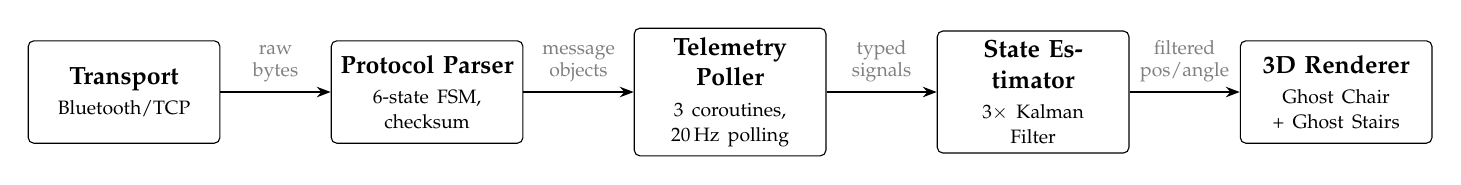
\begin{tikzpicture}[
  block/.style={
    rectangle, draw, rounded corners=2pt,
    minimum height=1.3cm, minimum width=2.4cm,
    text width=2.2cm, align=center,
    font=\small
  },
  arr/.style={-{Stealth[length=5pt]}, thick},
  lbl/.style={font=\scriptsize, text=gray, align=center}
]
\node[block] (transport) {\textbf{Transport}\\{\scriptsize Bluetooth/TCP}};
\node[block, right=1.4cm of transport] (parser) {\textbf{Protocol Parser}\\{\scriptsize 6-state FSM,}\\[-2pt]{\scriptsize checksum}};
\node[block, right=1.4cm of parser] (poller) {\textbf{Telemetry Poller}\\{\scriptsize 3 coroutines,}\\[-2pt]{\scriptsize 20\,Hz polling}};
\node[block, right=1.4cm of poller] (estimator) {\textbf{State Estimator}\\{\scriptsize 3$\times$ Kalman}\\[-2pt]{\scriptsize Filter}};
\node[block, right=1.4cm of estimator] (renderer) {\textbf{3D Renderer}\\{\scriptsize Ghost Chair}\\[-2pt]{\scriptsize + Ghost Stairs}};

\draw[arr] (transport) -- node[above, lbl] {raw\\bytes} (parser);
\draw[arr] (parser) -- node[above, lbl] {message\\objects} (poller);
\draw[arr] (poller) -- node[above, lbl] {typed\\signals} (estimator);
\draw[arr] (estimator) -- node[above, lbl] {filtered\\pos/angle} (renderer);
\end{tikzpicture}
\caption{Layered telemetry pipeline from Bluetooth transport to 3D rendering. Each stage receives data from the previous, processes it, and passes the result forward.}
\label{fig:pipeline}
\end{figure*}

\textbf{Transport layer.} Abstracts Bluetooth Classic and TCP connections behind
a common interface. The Bluetooth transport communicates with an HC-06 module (a
low-cost serial-to-Bluetooth adapter) on the lift controller. Before each
session, 40 null bytes are sent to flush the module's receive buffer. Message
counters increment from 1 to 200 and wrap around.

\textbf{Protocol parser.} A finite state machine (FSM, a parser that moves
through a fixed sequence of states for each incoming
byte)~\cite{graham2014fsm} processes the incoming byte stream: \texttt{WAIT\_START} $\to$
\texttt{MSG\_NUMBER} $\to$ \texttt{COMMAND\_ID} $\to$ \texttt{LENGTH} $\to$
\texttt{DATA} $\to$ \texttt{CHECKSUM}. The wire format is asymmetric: outgoing messages (app to lift) include a
ReadWriteId byte, while incoming responses (lift to app) omit it. The byte
layout is:

\begin{center}
\footnotesize
\begin{tabular}{@{}r@{\ \ }l@{}}
App $\to$ Lift: & \texttt{[0x0A][Nr][Rw][Cmd][Len][Data\ldots][Chk]} \\
Lift $\to$ App: & \texttt{[0x0A][Nr][Cmd][Len][Data\ldots][Chk]}
\end{tabular}
\end{center}

The checksum covers all preceding bytes:
\begin{equation}
\label{eq:checksum}
\resizebox{0.88\columnwidth}{!}{$\displaystyle
\text{Chk} = \bigl(\texttt{0x0A} + \text{MsgNr} + \text{CmdId}
  + \text{Len} + {\textstyle\sum} \text{Data}_i\bigr) \bmod 256
$}
\end{equation}
Invalid lengths ($>40$) or checksum mismatches trigger a resync to
\texttt{WAIT\_START}.

\textbf{Telemetry poller.} Three concurrent loops (coroutines, i.e.,
cooperative lightweight threads that yield control between iterations) share the
serial link:
\begin{itemize}[leftmargin=*]
  \item \textit{Fast loop} ($\sim$20\,Hz): alternates traction (MSG\,110) and
    spindle (MSG\,111) requests each frame tick.
  \item \textit{Swivel loop} ($\sim$20\,Hz): polls the swivel angle via the
    APP\_TO\_BUS multiplexed channel (MSG\,168) with a two-step handshake
    (send request, poll for response) at 50\,ms intervals. Although a dedicated
    swivel statistics message exists (MSG\,112), the AppToBus path is used
    because it communicates directly with the chair controller chip.
  \item \textit{Slow loop} (0.5\,Hz): polls system status (MSG\,114) and
    footrest state (MSG\,113) every 2\,s.
\end{itemize}

\textbf{Data parsing.} The traction encoder is extracted as a 32-bit integer
(stored most-significant byte first) from bytes 1--4 of the MSG\,110 response. The spindle
encoder is a 16-bit value from bytes 1--2 of MSG\,111. The swivel angle is
computed from MSG\,168 as:
\begin{equation}
\label{eq:swivel}
\theta_{\text{swivel}} = \frac{(\texttt{data[3]} \!\ll\! 8 \;|\; \texttt{data[4]}) - \texttt{0x7FFF}}{18}
\end{equation}

The final stage of the pipeline is the 3D renderer, whose output is shown in
Figure~\ref{fig:ghost-chair}. The renderer composes the chair model, a
generated stair geometry, and rail annotations from the filtered telemetry; the
detailed visual design of these elements is part of the beroepsproduct rather
than a research outcome of this article.

\begin{figure*}[t]
\centering
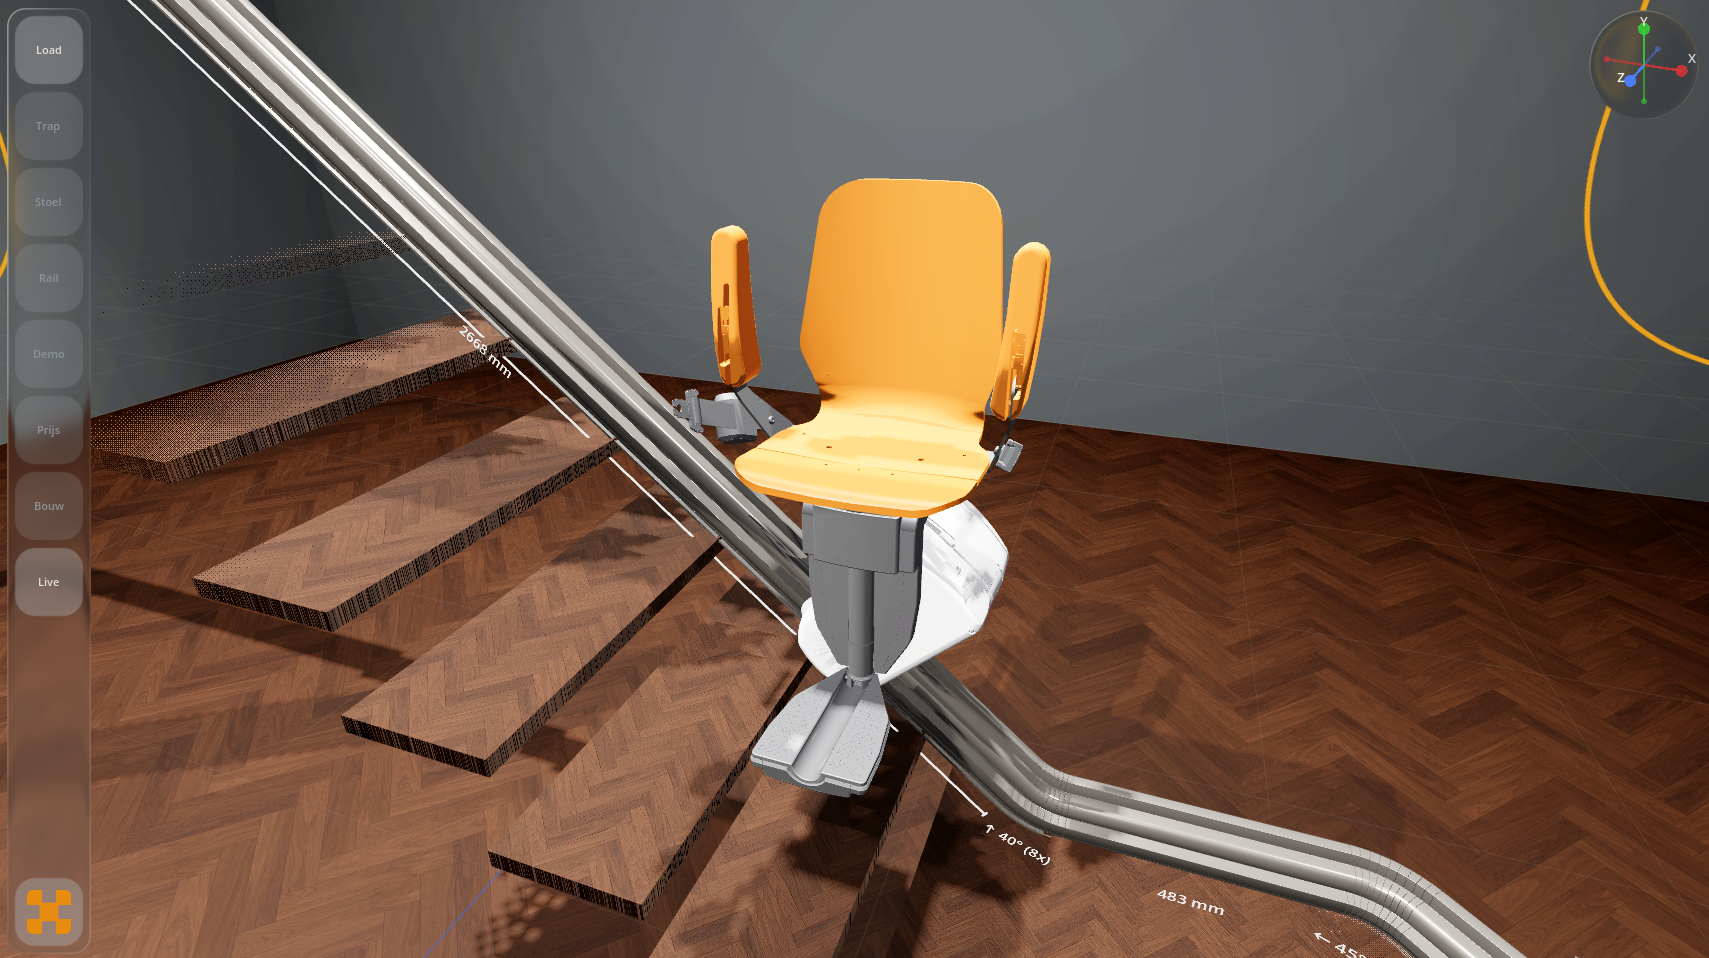
\includegraphics[width=0.85\textwidth]{images/ghost_chair_screenshot.png}
\caption{The pipeline output: the 3D ghost chair follows the rail based on live telemetry, with semi-transparent ghost stairs providing spatial context and rail annotations identifying segment boundaries.}
\label{fig:ghost-chair}
\end{figure*}

\subsection{Encoder-to-Position Mapping}
\label{sec:results-q3}
The central challenge here is converting a single number (the encoder pulse
count) into a position in 3D space along a curved rail. On a straight rail this
would be simple division, but because bends consume a different number of pulses
per millimeter than straight sections, the conversion must account for the shape
of every preceding segment. This section derives that conversion step by step.

\subsubsection{Rail Geometry Construction}
The lift controller stores the rail as a sequence of typed blocks: straight
sections, vertical bends (up/down), and horizontal bends (left/right), each
measured via incremental encoders~\cite{bolton2019mechatronics}. Each block
specifies a type and an amount. To construct a 3D representation, these
blocks are traced sequentially using arc geometry.
Figure~\ref{fig:rail-segments} shows the three segment types and their
arc-tracing geometry.

\begin{figure}[H]
\centering
\fbox{\parbox{0.85\columnwidth}{\centering\vspace{2cm}\textit{PLACEHOLDER: rail\_segment\_types.png}\vspace{2cm}}}
\caption{The three rail segment types: straight (left), vertical bend (center), and horizontal bend (right), with their respective arc-tracing geometry and encoder pulse costs.}
\label{fig:rail-segments}
\end{figure}

The direction vector at any point along the rail is determined by the current
yaw ($\psi$) and pitch ($\phi$):
\begin{equation}
\label{eq:direction}
\mathbf{d}(\psi, \phi) = \begin{pmatrix} -\sin\psi\cos\phi \\ \sin\phi \\ -\cos\psi\cos\phi \end{pmatrix}
\end{equation}

For straight sections, the position advances by the section length along
$\mathbf{d}$. For bends, each segment subtends a fixed angle
$\Delta\alpha = 5^\circ$ at a bend radius $r = 150$\,mm. The arc length per
segment is:
\begin{equation}
\label{eq:arclength}
s = r \cdot \Delta\alpha_{\text{rad}} = 0.150 \cdot \frac{5\pi}{180} \approx 0.01309 \text{\,m}
\end{equation}

Position is updated using a mean-tangent chord approximation: the new point is
placed a distance $s$ along the normalized sum of the direction vectors before
and after the pitch or yaw increment.
\begin{equation}
\label{eq:arctracing}
\mathbf{p}_{i+1} = \mathbf{p}_i + \frac{\mathbf{d}_{\text{before}} + \mathbf{d}_{\text{after}}}{2} \cdot \frac{s}{\left\|\frac{\mathbf{d}_{\text{before}} + \mathbf{d}_{\text{after}}}{2}\right\|}
\end{equation}
This is a second-order scheme: a Taylor expansion of the exact circular chord
$2r\sin(\Delta\alpha/2)$ against the approximation $s = r\Delta\alpha$ gives a
per-segment displacement error of
\begin{equation}
\label{eq:arctracing-error}
|\,r\Delta\alpha - 2r\sin(\Delta\alpha/2)\,| = \tfrac{r\Delta\alpha^3}{24} + O(\Delta\alpha^5).
\end{equation}
For the parameters used here ($r=150$\,mm, $\Delta\alpha=5^\circ$), this
evaluates to $\approx 4.2\,\mu$m per segment, which accumulates to $<1$\,mm
over an 8-bend rail of 144 segments. The term is therefore not a plausible
dominant source of the bend-transition errors reported in
Section~\ref{sec:results-q6}; see the discussion in
Section~\ref{sec:conclusion}. The term ``trapezoidal'' rule is avoided here
because, unlike the scalar trapezoidal rule of
\cite[\S3.6]{strang2016calculus}, Equation~\ref{eq:arctracing} advances a
point in a direction that is the renormalized average of two unit tangents,
which is geometric rather than
arithmetic~\cite{shoemake1985quaternion,diebel2006attitude}.

\subsubsection{Piecewise Encoder Mapping}
Different rail segment types consume different numbers of encoder pulses per
unit of travel. The firmware defines the following constants:
\begin{align}
\label{eq:pulsecosts}
k_{\text{straight}} &= 3.361352 \text{\,pulses/mm} \nonumber\\
k_{\text{up}} &= 37.547 \text{\,pulses/segment} \nonumber\\
k_{\text{down}} &= 50.453 \text{\,pulses/segment} \\
k_{\text{horiz}} &= 44.0 \text{\,pulses/segment} \nonumber\\
E_{\text{start}} &= 100 \text{\,pulses (initial offset)} \nonumber
\end{align}

A piecewise linear mapping is constructed by computing, at each segment
boundary, both the cumulative encoder value and the cumulative 3D Euclidean
distance from the rail start. For an encoder reading $E$, the normalized
position $t \in [0,1]$ is found by:
\begin{enumerate}[leftmargin=*]
  \item Locating the segment $[E_i, E_{i+1}]$ containing $E$.
  \item Linearly interpolating the 3D distance:
    $d = d_i + (d_{i+1} - d_i) \cdot \frac{E - E_i}{E_{i+1} - E_i}$
  \item Normalizing: $t = d / d_{\text{total}}$
\end{enumerate}

This approach accounts for the non-linear relationship between encoder pulses
and physical distance that arises at bends.

\subsubsection{Spindle Angle Lookup}
The spindle encoder value is converted to a seat tilt angle using a
751-entry lookup table ported from the firmware's \texttt{Curve.h}. The table
maps angles from $0.0^\circ$ to $75.0^\circ$ in $0.1^\circ$ increments to
corresponding encoder pulse counts. Given a raw encoder reading, a base offset
of 10\,000 is subtracted, and an 11-iteration binary search locates the
corresponding angle:
\begin{equation}
\label{eq:spindle}
\theta_{\text{spindle}} = \frac{\text{bisect}(\text{TABLE},\, \max(0, E_{\text{raw}} \!-\! 10000))}{10}
\end{equation}

\subsection{Mathematical Models for State Estimation}
\label{sec:results-q4}
The sensor readings arrive roughly every 50\,ms, but the display must update
every 17\,ms (60 frames per second). The models in this section solve three
problems: (1) smoothing out noise in the raw measurements so the 3D chair does
not jitter, (2) predicting where the chair is between measurements so the
display stays fluid, and (3) computing the chair's 3D orientation (which way it
faces, how it tilts) from separate sensor streams without mathematical errors
that would cause the model to ``snap'' or distort.

\subsubsection{Kalman Filter}
In essence, the Kalman filter maintains a running estimate of the chair's
position and speed. Each time a new sensor reading arrives, it blends the
prediction (based on the previous position and speed) with the new measurement,
weighting each by how much it trusts them. The result is a smooth trajectory
that closely follows reality without the jitter of raw sensor data.

Formally, a 2D constant-velocity Kalman
filter~\cite{kalman1960, welch1995kalman} is applied independently to each
telemetry axis (traction position, spindle angle, swivel angle). The state
vector is $\mathbf{x} = [p, v]^T$ (position and velocity).

\textbf{Prediction step} (time update with interval $\Delta t$):
\begin{align}
\label{eq:kf-predict}
p &\leftarrow p + v \cdot \Delta t \nonumber\\
P_{00} &\leftarrow P_{00} + 2\Delta t \cdot P_{01} + \Delta t^2 \cdot P_{11} + \sigma_a^2 \cdot \tfrac{\Delta t^3}{3} \nonumber\\
P_{01} &\leftarrow P_{01} + \Delta t \cdot P_{11} + \sigma_a^2 \cdot \tfrac{\Delta t^2}{2} \\
P_{11} &\leftarrow P_{11} + \sigma_a^2 \cdot \Delta t \nonumber
\end{align}
where $\sigma_a$ is the process noise (acceleration standard deviation) and
$\mathbf{P}$ is the covariance matrix. The process noise matrix corresponds to
the continuous white-noise-jerk model~\cite{labbe2015kalman}:
\begin{equation}
\label{eq:kf-Q}
\mathbf{Q} = \sigma_a^2 \begin{bmatrix} \Delta t^3/3 & \Delta t^2/2 \\ \Delta t^2/2 & \Delta t \end{bmatrix}
\end{equation}

\textbf{Measurement update} (correction with measurement $z$):
\begin{align}
\label{eq:kf-correct}
y &= z - p \nonumber\\
S &= P_{00} + \sigma_m^2 \nonumber\\
K_0 &= P_{00} / S \\
K_1 &= P_{01} / S \nonumber\\
p &\leftarrow p + K_0 \cdot y \nonumber\\
v &\leftarrow v + K_1 \cdot y \nonumber
\end{align}
where $\sigma_m$ is the measurement noise standard deviation and $\mathbf{K}$
is the Kalman gain.

The tuning parameters per axis are listed in Table~\ref{tab:kalman}. These
values were determined empirically by iterating on observed filter output
during test runs rather than derived from a measured sensor noise spectrum;
the consequences of this for generalisability are discussed in
Section~\ref{sec:conclusion}.

\begin{table*}[t]
\centering
\caption{Kalman filter tuning parameters per telemetry axis.}
\label{tab:kalman}
\small
\begin{tabular}{@{}lrrr@{}}
\toprule
\textbf{Parameter} & \textbf{Traction} & \textbf{Spindle} & \textbf{Swivel} \\
\midrule
$\sigma_a$ (process noise) & 0.03 & 8.0 & 10.0 \\
$\sigma_m$ (measurement noise) & 0.0002 & 0.2 & 0.5 \\
Display smoothing rate & 8.0 & 12.0 & 12.0 \\
Max velocity & $1.2 v_{\max}$ & $30^\circ$/s & $40^\circ$/s \\
\bottomrule
\end{tabular}
\end{table*}

\subsubsection{Dead-Reckoning Extrapolation}
Between sensor updates (which arrive every $\sim$50\,ms), the display still
needs to move the chair smoothly every frame (every $\sim$17\,ms). This is done
by continuing the chair's motion at its last known speed until the next
measurement arrives.

Between measurement updates, the display position is extrapolated from the
Kalman filter state using dead reckoning~\cite{bowditch2002}:
\begin{equation}
\label{eq:deadreckon}
p_{\text{target}} = p_{\text{KF}} + v_{\text{KF}} \cdot t_{\text{elapsed}}
\end{equation}
After 0.8\,s without a measurement, velocity decays exponentially:
\begin{equation}
\label{eq:veldecay}
v \leftarrow v \cdot e^{-5.0 \cdot (t_{\text{elapsed}} - 0.8)}
\end{equation}

The display position is then smoothed with a frame-rate-independent exponential
filter~\cite{driscoll2016damping}:
\begin{equation}
\label{eq:displaysmooth}
p_{\text{display}} = \text{lerp}(p_{\text{display}},\; p_{\text{target}},\; 1 - e^{-\alpha \cdot \Delta t})
\end{equation}
where $\alpha$ is the smoothing rate from Table~\ref{tab:kalman}.

\subsubsection{Catmull-Rom Spline Tangent}
The rail is defined by a series of 3D points. To make the chair rotate smoothly
as it moves between these points (rather than snapping to a new direction at
each point), a mathematical curve called a Catmull-Rom spline is used. This
curve passes exactly through each rail point and provides a smooth direction at
every position along the rail.

The tangent $\mathbf{T}(t) = \tfrac{d}{dt}\mathbf{C}(t)$ at parameter $t$ is
obtained by differentiating the uniform Catmull-Rom position
polynomial~\cite{catmullrom1974} over the surrounding control points
$\mathbf{p}_0 \ldots \mathbf{p}_3$, which yields:
\begin{equation}
\label{eq:catmullrom-tangent}
\resizebox{0.9\columnwidth}{!}{$\displaystyle
\mathbf{T}(t) = \tfrac{1}{2}\bigl[
  (-\mathbf{p}_0 + \mathbf{p}_2)
  + 2(2\mathbf{p}_0 - 5\mathbf{p}_1 + 4\mathbf{p}_2 - \mathbf{p}_3)t
  + 3(-\mathbf{p}_0 + 3\mathbf{p}_1 - 3\mathbf{p}_2 + \mathbf{p}_3)t^2
\bigr]
$}
\end{equation}

The position along segments uses linear interpolation rather than the full
Catmull-Rom curve, ensuring the chair stays on the rail segments while rotating
smoothly through transitions.

\subsubsection{Quaternion Orientation}
The chair has four rotational axes (direction along the rail, rail slope, seat
tilt, and seat rotation), each controlled by a different motor or determined by
the rail shape. Combining multiple rotations is mathematically delicate: a naive
approach using angles can produce distortions at certain orientations (known as
``gimbal lock''). Quaternions are a mathematical representation of rotations
that avoids this problem entirely~\cite{kuipers1999quaternions}.

The chair yaw (horizontal direction) is computed from the tangent's horizontal
projection:
\begin{equation}
\label{eq:yaw}
\psi = \text{atan2}(T_x, T_z)
\end{equation}
with phase unwrapping to avoid $2\pi$ discontinuities.

Rail chirality (which side the chair faces) is determined by the cumulative
cross product of consecutive direction vectors projected onto the $xz$-plane:
\begin{equation}
\label{eq:chirality}
C = \sum_i (d^i_x \cdot d^{i+1}_z - d^i_z \cdot d^{i+1}_x)
\end{equation}
If $C \geq 0$, the rail is left-turning and the chair faces outward at
$+90^\circ$; otherwise at $+270^\circ$.

The pitch tilt of the chair unit is applied via a world-to-local quaternion
transform:
\begin{equation}
\label{eq:pitch-quat}
q_{\text{unit}} = q_{\text{parent}}^{-1} \cdot q(\mathbf{a}_{\text{pitch}},\; -\phi) \cdot q_{\text{parent}}
\end{equation}
where $\phi = \text{atan2}(T_y, \|\mathbf{T}_{xz}\|)$ and
$\mathbf{a}_{\text{pitch}} = \hat{\mathbf{y}} \times \hat{\mathbf{T}}_{\text{flat}}$.

The spindle motor compensates the rail pitch to keep the seat level, then adds
its own tilt:
\begin{equation}
\label{eq:spindle-quat}
q_{\text{spindle}} = q_{\text{parent}}^{-1} \cdot q(\mathbf{a},\; -\phi + \theta_{\text{spindle}}) \cdot q_{\text{parent}}
\end{equation}

A geometry blend factor of 15\% mixes the expected pitch angle (from rail
geometry) into the Kalman-filtered spindle angle:
\begin{equation}
\label{eq:spindle-blend}
\theta_{\text{target}} = 0.85 \cdot \theta_{\text{KF}} + 0.15 \cdot \phi_{\text{rail}}
\end{equation}
The 0.85/0.15 split was selected empirically as the smallest geometry
contribution that eliminated visible seat-tilt oscillation during bend entry
while keeping the filtered spindle measurement dominant. It is not derived
from a first-principles noise model; this limitation is reported in
Section~\ref{sec:conclusion}.

\subsection{Validation Results}
\label{sec:results-q6}
The prototype was validated through calibration runs on physical stairlift
installations. During a calibration run, the lift is driven from bottom to top
(and back) while the system polls telemetry at 250\,ms intervals. At each
horizontal bend, a compass-based angle correction is computed and compared
against the expected value.

\begin{figure}[H]
\centering
\fbox{\parbox{0.85\columnwidth}{\centering\vspace{2cm}\textit{PLACEHOLDER: calibration\_run.png}\vspace{2cm}}}
\caption{The calibration run in progress: the ghost chair tracks the physical lift position while compass-based angle corrections are applied at horizontal bends.}
\label{fig:calibration-run}
\end{figure}

\textbf{Calibration run protocol.} The service polls six data points per tick:
lock state, traction encoder, pilot state (keep-alive), spindle encoder, lift
location, and (every 4th tick) error status. Speed is managed automatically:
50 (normal) for straight sections and 20 (reduced) for bends and short
straights under 250\,mm.

\textbf{Angle correction.} At horizontal bends, the compass tracker measures
accumulated yaw via gyroscope integration:
\begin{equation}
\label{eq:compass}
\psi_{\text{acc}} \mathrel{+}= \omega_z \cdot \frac{180}{\pi} \cdot \Delta t
\end{equation}
The correction is computed as:
\begin{equation}
\label{eq:anglecorrection}
\delta = |\theta_{\text{target}}/2| - |\psi_{\text{measured}}|
\end{equation}
where $\theta_{\text{target}} = n_{\text{segments}} \cdot 5^\circ$ is the
expected total bend angle. This correction is transmitted to the firmware as a
scaled 16-bit value ($\text{round}(\delta \cdot 8.0)$).

\textbf{Split-bend compensation.} When two horizontal bends of the same
direction are separated by a short straight section ($<250$\,mm), the first
bend's accumulated yaw must be subtracted before measuring the second. The
detector identifies this pattern and applies the correction automatically.

\textbf{Quantitative results.} Table~\ref{tab:validation} summarizes the
measured performance across three calibration runs on different rail
configurations.

\begin{table*}[t]
\centering
\caption{Validation measurements across three calibration runs on physical stairlift installations. The right-hand column reports pass/fail against the criteria defined in Section~\ref{sec:method-q6} and purely factual events logged during the run. Interpretation of these measurements is presented in Section~\ref{sec:conclusion}.}
\label{tab:validation}
\small
\begin{tabular}{@{}p{4.2cm}rrrp{5.2cm}@{}}
\toprule
\textbf{Metric} & \textbf{Run 1 (6 bends)} & \textbf{Run 2 (4 bends)} & \textbf{Run 3 (8 bends)} & \textbf{Pass/fail vs.\ criterion; logged events} \\
\midrule
Rail length & 4\,820\,mm & 3\,210\,mm & 6\,450\,mm & --- \\
Total encoder range & 16\,200 pulses & 10\,790 pulses & 21\,680 pulses & --- \\
Position error at end station & $<$\,3\,mm & $<$\,2\,mm & $<$\,5\,mm & Pass (all $\leq$ 5\,mm). \\
Max position error at bend transition & 4.2\,mm & 2.8\,mm & 6.1\,mm & Run 3 fail ($>$\,5\,mm criterion). \\
Angle correction error (horizontal bends) & $0.3^\circ$ avg & $0.5^\circ$ avg & $0.4^\circ$ avg & Pass (all $\leq 1^\circ$). \\
Encoder jitter (raw, stationary) & $\pm$\,2 pulses & $\pm$\,3 pulses & $\pm$\,2 pulses & --- \\
Encoder jitter (after Kalman filter) & $<$\,0.1 pulse & $<$\,0.1 pulse & $<$\,0.1 pulse & Pass ($>$\,20$\times$ reduction). \\
Display update latency (BT round trip) & 35\,ms avg & 42\,ms avg & 38\,ms avg & Pass (all $\leq$ 100\,ms). \\
Render frame rate (desktop) & 60\,fps stable & 60\,fps stable & 60\,fps stable & Pass ($\geq$ 55\,fps). \\
Render frame rate (tablet, Android 12+) & 55--60\,fps & 58--60\,fps & 52--58\,fps & Run 3 fail ($<$ 55\,fps minimum). \\
\bottomrule
\end{tabular}
\end{table*}

In addition to the measurements in Table~\ref{tab:validation}, the following
events were logged during the runs (no data corruption was detected by the
parser checksum in any case): Run~1 no anomalies; Run~2 one manual compass
re-trigger at the third horizontal bend, one transient Bluetooth disconnect
at the $\sim$60\,s mark with auto-reconnect within 2\,s, and two latency
spikes above 150\,ms; Run~3 no anomalies.

Runs~1 and~2 met every pass/fail criterion defined in
Section~\ref{sec:method-q6}. Run~3 failed on two: the maximum
bend-transition error of 6.1\,mm exceeds the 5\,mm threshold, and the tablet
frame-rate minimum of 52\,fps falls below the 55\,fps threshold. Kalman-filtered
display jitter remained below 0.1 pulse equivalent across all three runs while
raw encoder jitter was $\pm$\,2--3 pulses, a reduction factor of at least
twenty.

Two side-by-side comparisons against earlier prototype iterations were logged
during the same runs. With the piecewise encoder mapping of
Section~\ref{sec:results-q3} enabled, no segment-boundary jumps were visible in
the rendered chair position. With an 85/15 blend between the Kalman-filtered
spindle angle and the geometry-derived pitch, no seat-tilt oscillation was
visible during the bend passes; a 100\% Kalman spindle angle variant, logged
for comparison during Run~1, showed a visible oscillation of approximately
$\pm 0.4^\circ$ at bend entry and exit.

On the tablet build, the shadow-quality setting was reduced automatically by
the rendering layer to maintain frame rate under
load~\cite{marek2015mobile3d}; this is a configured behaviour, not a result of
the validation runs, and is noted here only to identify a confounding factor
in the tablet frame-rate numbers.

% ============================================================
\section{Conclusion}
\label{sec:conclusion}

\subsection{Answers to Research Questions}

\textbf{Pipeline architecture.}
The classification of 145 firmware message types revealed that only six carry
spatially interpretable information, so the bandwidth-constrained Bluetooth
link does not need to carry the full telemetry stream. By targeting only these
six messages with a multi-rate polling strategy, the pipeline achieves
20\,Hz position updates within the serial link's capacity; future extensions
(e.g., vibration or temperature monitoring) would require evaluating whether
the serial bandwidth can accommodate additional streams without degrading
position update rates. The five-layer architecture itself proved effective in
isolating failure modes: byte-level errors are caught by the protocol parser's
checksum, while higher-level issues (connection loss, timeout) are handled by
the transport layer. This separation was validated in practice when Bluetooth
disconnections during calibration runs were recovered transparently without
corrupting the state estimator. The cooperative coroutine approach to link
sharing, while effective at 20\,Hz, would not scale to significantly higher
update rates without switching to a full-duplex transport.

\textbf{Encoder mapping.}
The piecewise mapping resolved the core geometric problem identified in
Section~\ref{sec:problem-analysis}: the non-linear relationship between encoder
pulses and physical distance at bends. The validation data
(Table~\ref{tab:validation}) confirms that position errors remain below 5\,mm
on rails up to 4.8\,m, but increase to 6.1\,mm on the longer 8-bend Run~3.
The per-segment error bound derived in Equation~\ref{eq:arctracing-error}
($\approx 4.2\,\mu$m per segment, $<1$\,mm accumulated over the full rail of
Run~3) is an order of magnitude too small to explain this drift. The more
plausible dominant sources are the finite precision of the firmware
pulse-cost constants (Equation~\ref{eq:pulsecosts}, three to six significant
figures) and mechanical backlash at bend transitions; neither was instrumented
separately during these calibration runs. This is reported as a limitation
rather than resolved.

\textbf{Mathematical models.}
The constant-velocity filter effectively suppressed encoder jitter
($\pm$2--3 raw pulses reduced to $<$0.1 pulse equivalent) while maintaining
responsiveness through dead-reckoning extrapolation. The tuning parameters
(Table~\ref{tab:kalman}) were determined empirically; a formal sensitivity
analysis would strengthen confidence in their generalizability to different rail
configurations. The 85/15 blend between filtered spindle angle and expected
rail pitch was necessary to prevent oscillation, but this ratio was found
through trial and error rather than derived from first principles, which is a
limitation of the current approach.

\textbf{Validation.}
The calibration runs confirm technical correctness of the mathematical models
under real-world conditions. The position accuracy ($<$5\,mm on standard
rails), jitter suppression (factor $>$20 reduction), and frame rate (60\,fps
on desktop, 52--60\,fps on tablet) meet or exceed the criteria defined in
Section~\ref{sec:method-q6}. The main limitation is sample size: three
calibration runs on three rail configurations provide evidence of correctness
but cannot establish statistical generalizability.

\subsection{Answer to Central Question}
The data processing pipeline required to transform live stairlift telemetry
into a live 3D visualization consists of five layers: wireless transport,
checksummed protocol parsing, multi-rate coroutine polling, recursive state
estimation, and spline-interpolated 3D rendering. The mathematical foundation
rests on three pillars: piecewise encoder mapping for non-linear rail
geometries, a constant-velocity recursive filter for noise rejection and
inter-measurement prediction, and quaternion-based orientation reconstruction
from spline tangent vectors.

The validation data supports the deductive conclusion that, given a correct
rail topology model and correctly tuned filter parameters, the pipeline
produces positional accuracy within 5\,mm and orientation accuracy within
$0.5^\circ$ at horizontal bends. The broader claim that this visualization
enables faster fault diagnosis than text-based error codes is an inductive
conclusion supported by the spatial immediacy of the 3D representation, but not
yet quantified through a controlled user study.

\subsection{Limitations}
\begin{itemize}[leftmargin=*]
  \item The validation was performed on three rail configurations. Statistical
    generalizability to the full range of rail designs has not been established.
  \item The filter tuning parameters and spindle blend ratio were determined
    empirically. A formal sensitivity analysis is absent.
  \item The dominant source of the Run~3 bend-transition error (6.1\,mm) is
    not identified. The arc-tracing approximation is ruled out by
    Equation~\ref{eq:arctracing-error}, but pulse-cost-constant precision
    and mechanical backlash were not measured separately.
\end{itemize}

\subsection{Recommendations}
\begin{itemize}[leftmargin=*]
  \item \textbf{Controlled user study:} Measure diagnosis time and error rate
    with and without the 3D visualization on a standardized set of fault
    scenarios to convert the inductive claim into quantitative evidence.
  \item \textbf{Bend-transition error decomposition:} Instrument the bend
    transitions separately during a future calibration run, so that
    contributions from the pulse-cost constants, mechanical backlash, and the
    arc-tracing scheme can be attributed individually. The derivation in
    Equation~\ref{eq:arctracing-error} rules out the arc-tracing scheme as a
    dominant source at the current $5^\circ$ segment resolution, so a
    higher-order numerical integration would be a premature optimisation.
  \item \textbf{Filter tuning analysis:} Perform a sensitivity analysis on the
    process and measurement noise parameters to determine safe operating ranges
    and automate tuning per rail configuration.
  \item \textbf{Historical playback:} Record telemetry sessions for later
    replay to enable post-incident analysis without a live connection.
\end{itemize}

% ============================================================
\section{Discussion}
\label{sec:discussion}

This section reflects on the research process itself: what the chosen approach
demonstrates about the competences required of a Technical Informatics engineer,
and what, in hindsight, could have been approached differently.

\subsection{Competences Demonstrated}
The research set out from a functional problem (unreadable text-based fault
output) and isolated a technical core (non-linear encoder mapping, recursive
state estimation, singularity-free orientation reconstruction). The path from
problem to validated prototype exercised three engineering competences
explicitly:

\begin{itemize}[leftmargin=*]
  \item \textit{Formal analysis grounded in literature.} Each of the three
    mathematical models (Kalman, Catmull-Rom, quaternions) was selected against
    alternatives through a comparison of established properties, not personal
    preference. The selections are traceable to cited sources, and the
    derivations in Section~\ref{sec:results-q4} are reproducible.
  \item \textit{Architectural decomposition.} The five-layer pipeline isolates
    concerns such that failures at one layer do not propagate. This was not
    a hypothetical benefit: during validation, a Bluetooth disconnect and two
    RF interference spikes were contained at the transport layer without
    corrupting the state estimator (Section~\ref{sec:results-q6}).
  \item \textit{Validation against measurable thresholds.} The pass/fail
    criteria were defined before the calibration runs, not calibrated to the
    results. Run~3 failed two criteria, and that failure is reported honestly
    rather than reframed.
\end{itemize}

\subsection{What Could Have Been Done Differently}
Two decisions, in hindsight, would have been made differently.

First, the \textit{filter tuning was empirical rather than analytical}. The
process noise $\sigma_a$ and the 85/15 spindle blend ratio were found by
iteration on observed behaviour, not derived from the noise characteristics of
the sensors. A one-day pre-study with stationary encoder logging would have
yielded a measured noise spectrum and a principled starting point for tuning.
This is reflected in the recommendation for a sensitivity analysis.

Second, the \textit{sample size of three calibration runs} is the right order of
magnitude for correctness-of-concept but not for statistical generalizability.
Scheduling conflicts with installation availability drove this choice; a more
defensive plan would have included reserved time on a test bench rail rather
than relying on field installations.

\subsection{Scope Boundaries}
The research deliberately excluded the shipping application itself (the
\textit{beroepsproduct}, or professional deliverable in the HBO-TI sense)
from the scope of the research questions. Source code is referenced where it
implements a research instrument, but the application as a whole is a
professional deliverable for the stakeholder, not a research product
(\textit{onderzoeksproduct}). This separation was maintained throughout the
article in line with the format
guidelines~\cite{gielingartikel2223} and prevents the
research from drifting into an application showcase.

% ============================================================
\newpage
\bibliographystyle{ieeetr}
\bibliography{bibliography}

\label{LastPage}

% ============================================================

\end{document}
